\documentclass{article}
\usepackage{subcaption}
\usepackage[french]{babel}
\usepackage[utf8]{inputenc}
\usepackage{graphicx}
\usepackage[justification=centering]{caption}

%%%%%%%%%%%%%%%% Lengths %%%%%%%%%%%%%%%%
\setlength{\textwidth}{15.5cm}
\setlength{\evensidemargin}{0.5cm}
\setlength{\oddsidemargin}{0.5cm}

%%%%%%%%%%%%%%%% Variables %%%%%%%%%%%%%%%%
\def\projet{1}
\def\titre{Représentation des nombres en machine }
\def\groupe{4}
\def\equipe{5}
\def\responsible{}
\def\secretary{}
\def\others{}

\begin{document}


%%%%%%%%%%%%%%%% Header %%%%%%%%%%%%%%%%
\noindent\begin{minipage}{0.98\textwidth}
  \vskip 0mm
  \noindent
  { \begin{tabular}{p{7.5cm}}
      {\bfseries \sffamily
        Projet \projet} \\ 
      {\itshape \titre}
    \end{tabular}}
  \hfill 
  \fbox{\begin{tabular}{l}
      {~\hfill \bfseries \sffamily Groupe \groupe\ - Equipe \equipe
        \hfill~} \\[2mm] 
      Responsable : \responsible \\
      Secrétaire : \secretary \\
      Codeurs : \others
    \end{tabular}}
  \vskip 4mm ~

  ~~~\parbox{0.95\textwidth}{\small \textit{Résumé~:} \sffamily Ce projet consiste à explorer les problèmes de précision qui peuvent survenir dans les calculs avec des nombres flottants en informatique. Il se concentre sur les opérations élémentaires et les algorithmes complexes pour montrer comment les erreurs peuvent apparaître dans les résultats. }
  \vskip 1mm ~
\end{minipage}


\section*{Introduction}
Les nombres à virgule flottante sont fréquemment utilisés pour les calculs mais peuvent entraîner des erreurs. Ce rapport examine les problèmes liés aux opérations sur des nombres à virgule flottante en se concentrant sur les erreurs des opérations élémentaires et les algorithmes pour gérer les erreurs de précision. Les deux aspects seront étudiés pour donner une compréhension complète des problèmes liés aux nombres à virgule flottante et comment les gérer.
\section{Représentation des nombres en machine}
L'objectif de cette partie est de simuler la représentation d'un nombre et les opération usuelles sur une machine, et visualiser la variation des erreurs du à ses opérations.
\subsection{Travail réalisé}
Dans cette partie du TD, nous avons à l'aide d'une fonction Python simuler la représentation des nombres en machine avec une précision donnée au sens de la Norme IEEE 754. Nous avons ensuite simuler les erreurs relatives à l'addition et multiplication des nombres en machine. Enfin nous avons étudier l'évolution des erreurs relatives pour les différentes opération pour un certain nombre donné.
\subsection{Description algorithmique}
\paragraph{Calcul de la représentation décimale réduite\\} 
Nous souhaitons calculer la représentation décimale réduite d'un nombre donné avec une certaine précision . Pour cela, Nous avons programmé la fonction rp(x,p) qui retourne la représentation décimale réduite du réel x avec la précision p. l'algorithme de la fonction consiste à trouver la notation scientifique du nombre x pour ensuite en tirer un nombre former par les p+1 premiers chiffre constituant la mantisse, on arrondie finalement ce nombre pour obtenir le résultat voulue. Cet algorithme peut \^etre résumer en les étapes suivante :
\begin{enumerate}
    \item $ n \leftarrow 0$,tant que $ \lfloor x \rfloor \notin [|1 , 9|] $ :
     \begin{itemize}
         \item si $ x < 1$ : $ x \leftarrow x*10$ et on incrémente n de 1
         \item si  $x>1$ : $x \leftarrow \frac{x}{10}$ et on décrémente n de 1
     \end{itemize}
     \item $x \leftarrow x*10^{p}$
     \item $ x \leftarrow arrondir\_unite(x)$
     \item  retourner $x*10^{-(p+n)}$
\end{enumerate}

La complexité temporelle de cette algorithme est linéaire en n l'exposant de x en sa notation scientifique, quant à la complexité spatiale elle reste constante.
\paragraph{Calcul des erreurs relatives\\}
Afin de calculer les erreurs relatives pour les opérations d'addition et multiplication nous avons simulé ses opérations en machine grâce à la fonction précédente, le calcul se fait ensuite directement par les formules données :
\begin{equation}
    \sigma_{add} (x,y) = \frac{|rp(x+y) - (x+y)|}{|x+y|}   
\end{equation}
\begin{equation}
    \sigma_{mult} (x,y) = \frac{|rp(x*y) - (x*y)|}{|x*y|}
\end{equation}

\subsubsection{Analyse des résultats}
Afin de comprendre l'évolution des erreurs relatives, Nous fixons un nombre réel $x=0.0001857563$ et nous évaluant en y les deux fonctions précédente sur un intervalle donnée avec une précision de 6 décimale.
\begin{figure}[!ht]
    \centering
    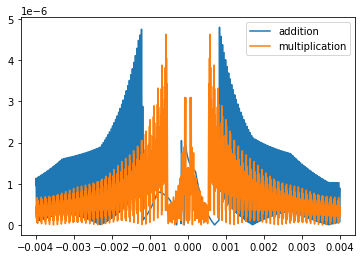
\includegraphics[width=60mm,scale=1.5]{res/graphe_fcts_erreur.png}
    \caption{Graphe des fonctions d'erreurs relatives d'addition et de multiplication pour $x=0.0001857563$ }
    \label{fig:graphe_erreur}
\end{figure}
\paragraph{Erreur relative d'addition\\}
En analysant la courbe bleue de la figure~\ref{fig:graphe_erreur}, représentant la fonction  $y \mapsto   \sigma_{add} (x,y) $ sur l'intervalle $[-0.004,0.004]$, nous remarquons que l'erreur est maximale pour $ |y| \simeq |x|$ mais reste limitée par la précision de la machine $10^{-6}$. Cela peut e\^tre justifier par le fait que l'erreur relative d'addition est traduit par un ajout des erreurs globales des termes de l'addition.


\paragraph{Erreur relative de multiplication\\}
La courbe orange de la figure~\ref{fig:graphe_erreur} représente la fonction $y \mapsto \sigma_{mult} (x,y) $ sur l'intervalle $[-0.004,0.004]$. On remarque dans ce cas que l'erreur relative est toujours majorée par la précision de la machine et décroît en s'éloignant de x. Cela est du au fait que l'erreur relative d'addition se traduit par un ajout des erreurs relatives des termes du produit. 

\section{Partie 2}
Dans cette partie nous allons étudier des méthodes de calcul qui couvre le besoin d'un calcul de basse précision.
\subsection{Travail réalisé}


\begin{itemize}
\item{Question 1}

Les nombres sur une calculatrice sont représentés en virgule flottante (=en utilisant une mantisse et un exposant). L'avantage principal de cette représentation est qu'elle permet de stocker beaucoup de nombres avec une grande précision. Mais elle peut également entraîner une perte de précision pour les nombres très grands ou très petits.
\item{Question 2}

La calculatrice stock des résultats précalculés et décompose chaque nombre donné de façon à le calculer avec ces valeurs déjà enregistrés. Par exemple, pour calculer ln(x) il faut voir que $x= (1+1)^{n0}*(1+1/10)^{n1}*...(1+1/10^6)^{n6}*(1+eps.)$ puis on composant par le ln et en utilisant ses propriétés on retrouve : $ln(x)= n0*ln(1+1)+n1*ln(1+1/10)+... +ln(1+eps.)$. En ce qui concerne le calcul des composantes n* l'agorythme se charge de les trouver selon la fonction utilisée.

Cette façon de calculer les images des fonctions permet de minimiser le poids dû calcule puisque la calculatrice est supposée être petite avec des processeurs pas trop puissants et une source d'énergie très limitée.
\item{Question 3}

La technique principale utilisée pour la mise en œuvre des algorithmes est appelée CORDIC. Elle implique une série de rotations dans le système de coordonnées pour évaluer rapidement des fonctions telles que lelogarithme népérien, l'exponentielle, l'arctangente et la tangente. Le processus consiste à effectuer des transformations simples, telles que des opérations d'addition/soustraction et de décalage, pour réduire la valeur d'entrée à un niveau très faible tout en déterminant le résultat. Des valeurs précalculées pour la fonction ou son inverse sont utilisées pour cela. Le résultat final est obtenu par interpolation linéaire ou une expansion en série.\\
Cette méthode est efficace pour les calculatrices car il nécessite peu de ressources matérielles, est facile à implémenter et offre des résultats précis avec une faible consommation d'énergie. Cela le rend particulièrement adapté aux périphériques de petite taille alimentés par des batteries.
\\


\begin{figure}[!h]

    \begin{minipage}[c]{.46\linewidth}
        \centering
        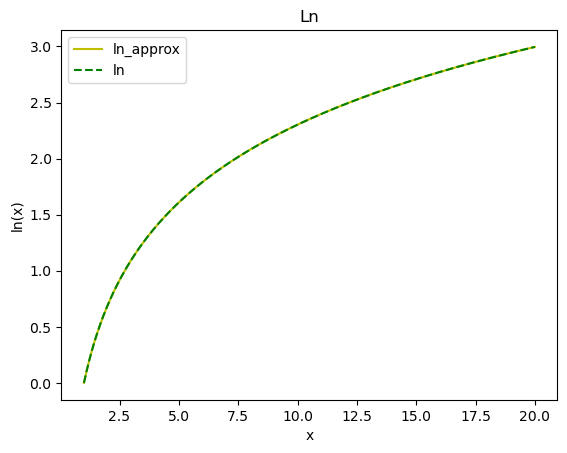
\includegraphics[width=50mm,scale=1.5]{res/ln_far.png}
        \caption{Graphe de ln et ln\_approx}
        \label{fig:graphe_ln}
    \end{minipage}
    \begin{minipage}[c]{.46\linewidth}
        \centering
        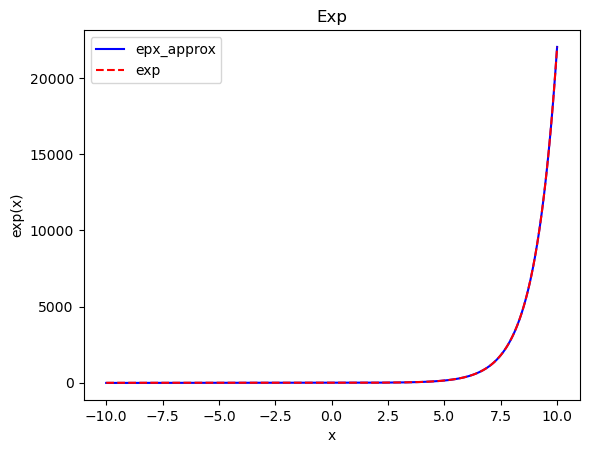
\includegraphics[width=50mm,scale=1.5]{res/exp_far.png}
        \caption{Graphe de exp et exp\_approx}
        \label{fig:graphe_exp}
    \end{minipage}
\end{figure}


\begin{figure}[!h]
    \begin{minipage}[c]{.46\linewidth}
        \centering
        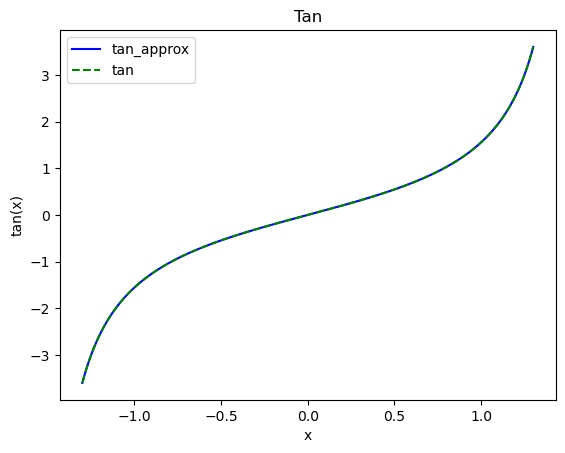
\includegraphics[width=50mm,scale=1.5]{res/tan_far.png}
        \caption{Graphe de tan et tan\_approx}
        \label{fig:graphe_tan}
    \end{minipage}
    \begin{minipage}[c]{.46\linewidth}
        \centering
        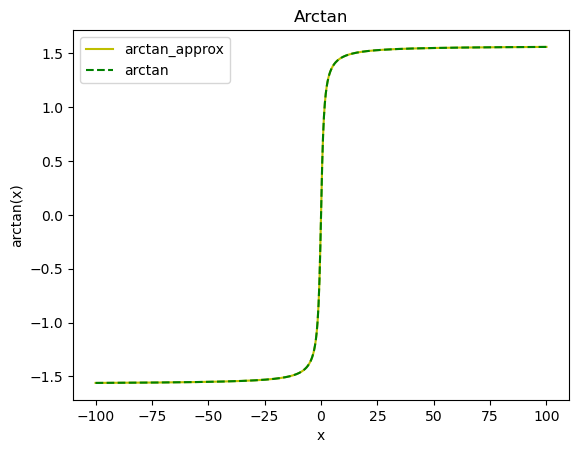
\includegraphics[width=50mm,scale=1.5]{res/arctan_far.png}
        \caption{Graphe de arctan et arctan\_approx}
        \label{fig:graphe_arctan}
    \end{minipage}
\end{figure}

\item{Question 4}

(Voir Analyse des résultats)
\end{itemize}


\subsection{Description algorithmique}

Ce code définit quatre fonctions mathématiques : le logarithme népérien (ln), l'exponentielle (exp), la tangente (tan) et l'arc tangente (arctan).\\

La fonction logarithme népérien utilise une boucle pour trouver une valeur approchée du logarithme en utilisant une liste précalculée de valeurs (L) qui contient des valeurs logarithmiques. Pour trouver la valeur approchée, la fonction compare la valeur d'entrée (x) à un produit de puissances de 10 et additionne les valeurs correspondantes de la liste L jusqu'à ce que la valeur d'entrée soit inférieure à ce produit. La fonction retourne finalement la somme des valeurs trouvées plus la division de x par le produit trouvé.\\

La fonction exponentielle utilise une boucle similaire à celle de la fonction logarithme népérien pour trouver une valeur approchée de l'exponentielle en utilisant toujours la liste L. La fonction compare la valeur d'entrée (x) à la liste L et soustrait la valeur correspondante jusqu'à ce que x soit inférieur à la valeur restante. La fonction retourne finalement la somme des valeurs trouvées multipliée par x.\\

La fonction arc tangente utilise une série de tests pour déterminer si x est négatif, supérieur à 1, égal à 0 ou égal à 1. Ensuite, la fonction utilise une boucle pour trouver une valeur approchée de l'arc tangente en utilisant une liste précalculée de valeurs (A) qui contient des valeurs arc tangentes. La fonction compare x à la liste A et additionne les valeurs correspondantes jusqu'à ce que x soit inférieur à la valeur restante. La fonction retourne finalement la somme des valeurs trouvées plus la division de x par la valeur restante.\\

La fonction tangente utilise une série de tests pour déterminer si x est négatif, supérieur à $\pi$, compris entre 0 et $\pi/2$, ou compris entre $\pi/2$ et $\pi/4$. Ensuite, la fonction utilise une boucle pour trouver une valeur approchée de la tangente en utilisant la liste A. La fonction compare x à la liste A et additionne les valeurs correspondantes jusqu'à ce que x soit inférieur à la valeur restante. La fonction retourne finalement la division de la somme des valeurs trouvées par la somme des valeurs complémentaires, divisée par la différence entre la somme des valeurs complémentaires et la multiplication de x par la somme des valeurs trouvées.\\

\subsection{Analyse des résultats}
On remarque que les graphes sont confondus d'après les figures \ref{fig:graphe_ln} \ref{fig:graphe_exp} \ref{fig:graphe_tan} \ref{fig:graphe_arctan}.
Mais pour être sur il faut calculer les différences entre les valeurs en chaque point.

Ce calcul donne le graphe suivant \ref{fig:erreurs}, on remarque effectivement que les valeurs sont presque egales à $~10^{-11}$ ce qui veux dire que nos valeurs par les fonction {ln, exp, tan, arctan} sont différentes à partir de la puissance -11 pour \ref{fig:graphe_ln} \ref{fig:graphe_tan} et \ref{fig:graphe_arctan}. Par contre on vois clairement que la valeurs de l'erreur en exponentielle diverge quand  $x \to-\infty$.

On pense que ceci vient du faite que la valeur de en ces point en coposant par la fonction exp est plus petit que epsilon tolérée par python. $(\lim_{x \to -\infty} exp(x) =0)$


\begin{figure}[!h]
    \centering
    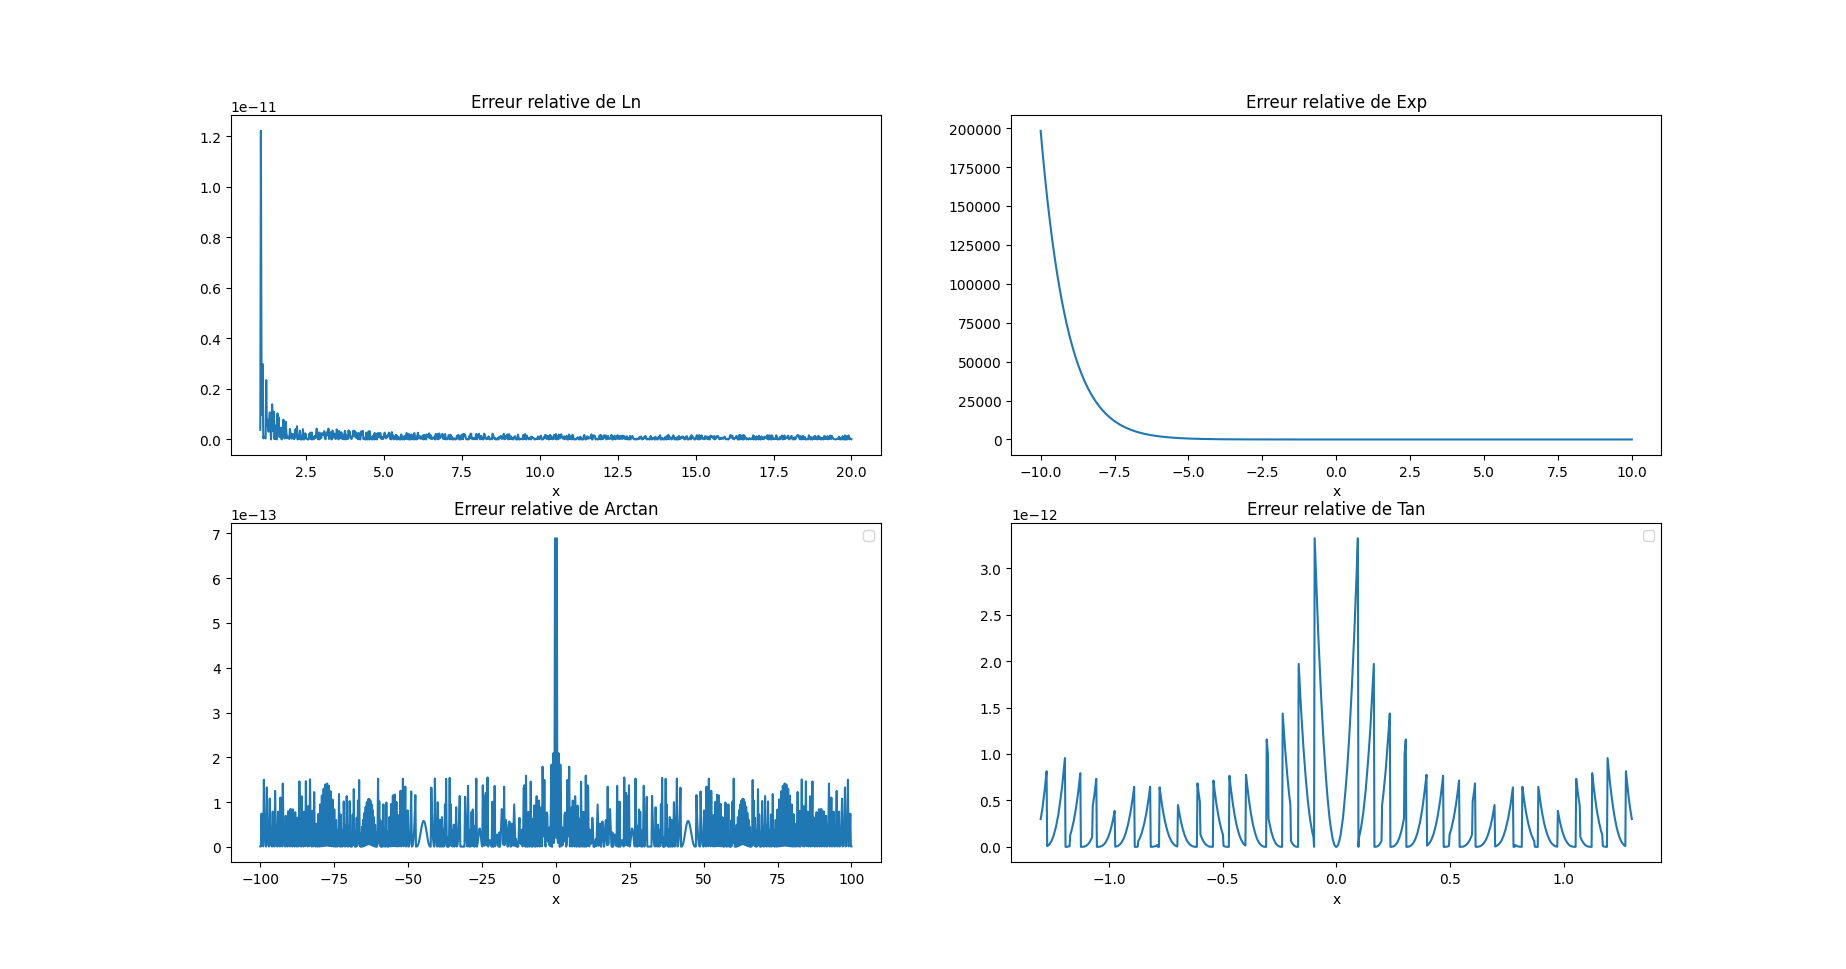
\includegraphics[width=200mm,scale=1.5]{res/Erreur_relative_p2.png}
    \caption{Graphes des erreurs de calculs}
    \label{fig:erreurs}
\end{figure}

\end{document}

